\begin{adjustbox}{width=\textwidth}
	\begin{tikzpicture}[every node/.style={inner sep=0,outer sep=0}]
	
		\node [anchor=north east] (img1) at (-0.03\textwidth,0) {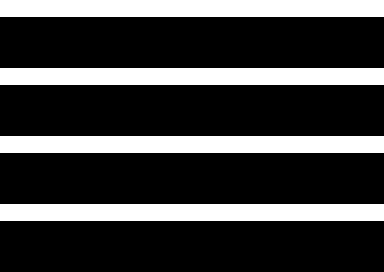
\includegraphics[frame,width=.47\textwidth]{03_sichtpruefungDurchLichtstreuung/optimierungen/musterMitUnterschiedlichenStreifenbreiten/figures/impulsStreifenmuster}};
		\node [below=0.2cm of img1] {Muster $m_1$ mit $\psi_1 = 0$};
		\node [anchor=north west] (img2) at (0.03\textwidth,0) {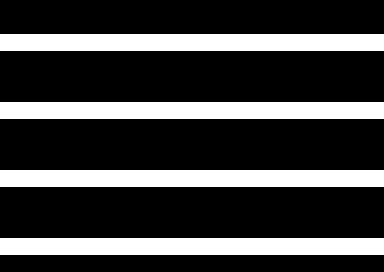
\includegraphics[frame,width=.47\textwidth]{03_sichtpruefungDurchLichtstreuung/optimierungen/musterMitUnterschiedlichenStreifenbreiten/figures/impulsStreifenmuster_shifted}};
		\node [below=0.2cm of img2] {Muster $m_3$ mit $\psi_3 = \pi$};
		
	\end{tikzpicture}
\end{adjustbox}
\caption[Streifenmuster durch Impulsschwingung]{Horizontale Streifenmuster analog zu Gleichung \ref{eq:impulsStreifenmuster} erzeugt, mit $A_m = 127.5$, $N_p = 4$, $\acrshortmath{lheight} = 272$, $N_{shift} = 4$ und $D = \tfrac{1}{4}$. Die hellen Streifen haben damit eine Höhe von 17 Pixeln und die dunklen Streifen eine Höhe von 51 Pixeln.}